%%%%%%%%%%%%%%%%%%%%%%%%%%%%%%%%%%%%%%%%%%%%%%%%%%%%%%%%%%%%%%%%%%%%%%%%%%%%%%%%
%2345678901234567890123456789012345678901234567890123456789012345678901234567890
%        1         2         3         4         5         6         7         8

\documentclass[letterpaper, 10 pt, conference]{ieeeconf}  % Comment this line out
                                                          % if you need a4paper
%\documentclass[a4paper, 10pt, conference]{ieeeconf}      % Use this line for a4
                                                          % paper

\IEEEoverridecommandlockouts                              % This command is only
                                                          % needed if you want to
                                                          % use the \thanks command
\overrideIEEEmargins
% See the \addtolength command later in the file to balance the column lengths
% on the last page of the document

\usepackage{graphicx}
\usepackage{subfigure}
\usepackage[]{units}
\usepackage{url}
\usepackage{mathtools}

\title{\LARGE \bf
Analysis of Current Data Mining Techniques on SMS Spam Filtering
%I Got Them Research Paper Writing Blues...
%Intoxicated Cells: a Prospective Study of the Effects of Tequila on Pluripotent Stem Cells
}

\author{William Marshall$^1$%
%\thanks{*This work was supported by SUNFEST}% <-this % stops a space
\thanks{$^2$Lehigh University, USA {\tt\small wcm214@lehigh.edu}}
}

\begin{document}
\maketitle
\thispagestyle{empty}
\pagestyle{empty}


%%%%%%%%%%%%%%%%%%%%%%%%%%%%%%%%%%%%%%%%%%%%%%%%%%%%%%%%%%%%%%%%%%%%%%%%%%%%%%%%
\begin{abstract}
The necessity of a fast, accurate, easily trainable spam detection
system is reflected in the current proliferation of SMS spam
messages. By taking advantage of the suite of machine learning
algorithms integrated into WEKA, we provide an analysis of SMS spam
detection accuracy across severak different learning models, and
present the Naive Bayes algorithm as a primary choice.
\end{abstract}


%%%%%%%%%%%%%%%%%%%%%%%%%%%%%%%%%%%%%%%%%%%%%%%%%%%%%%%%%%%%%%%%%%%%%%%%%%%%%%%%
\section{INTRODUCTION}
Short Message Service (SMS) messages are one of the primary means of
communication. Between the years of 2007 and 2010, the number of sent
SMS messages tripled, and the global rate of message sending increased
to 200,000 texts per second [1]. Along with the increased usage of SMS
messages, the proportion of SMS spam messages has also not only risen
to match the new levels of traffic, but has accelerated to the point
where parts of Asia classified 30\% of all SMS messages as spam in
2012 [2]. Although SMS spam is not as prevelant as email spam -- which
constituted 70.7\% of all emails in Q2 2013 -- there is still a strong
motivation for cellular companies to employ effective spam detection
systems, since it's likely that customers are willing to pay more for
a service that is insulated from spam.

Many modern approaches to spam detection are founded upon the research
that stems from the identification of email spam. Email spam detection
benefits from features such as a subject header, initial greetings,
and the IP address of the sender. Such features are not applicable to
SMS messages which have an upper limit of 160 characters, providing
overall less information to perform classification. Additionally,
since SMS spam is less pervasive than email spam, its classification
is made more difficult due to the lower prior probability. Blanzieri
at al. were able to achieve an email spam misclassification rate of
only 1.17\% [3], which is a daunting task for SMS spam detection.

The differences between SMS and email spam detection warrant a
reevaluation of the effectiveness of current learning
models. Fortunately, the University of Waikato has provided WEKA: a
toolkit that conveniently provides implementations of many well known
and vetted classification, association, and clustering techniques. The
algorithms included in WEKA and tested in this paper are by no means
an exhaustive analysis of the spam detetion literature, yet this paper
should function well as an introduction for those who are new to
machine learning, WEKA, and spam detection.

\section{Dataset}
The dataset in question was collected from the UCI Machine learning
repository,which contains 5574 text messages, 425 ofwhich were spam,
the rest of which are non-spam. This dataset was chosen because its
spam to non-spam ratio of 7.6\% roughly approximates the SMS spam rate
found in nature, since the spam rate in the UK is around 20\% [6],
while the SMS spam rate inthe US is less than 1\%. The data was
collected from a website called grumbletext.com,where users post the
text of spam messages that they have recieved, and was manually
inspected and classified.

It should be noted that there is an inherent bias in the dataset,
since the messages were collected from cellular users in the United
Kingdom. As a result of this, certain features that are a strong
indicator of spam (such as the presence of the ``£'' character) are
not as applicable to messages recieved in the United States. Such
geographic, culture, and language-based biases are unavoidable, and
actual implementations of the following learning models would do well
to train on messages from the intended location.

\section{Preprocessing}
\begin{figure}[t]
\centering
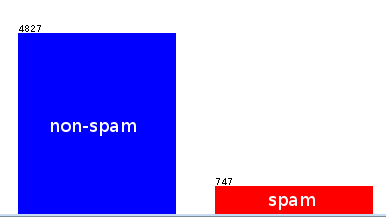
\includegraphics[width=0.9\columnwidth]{figures/spam_ham.png}
\caption{ The SMS spam detectin system is trained on a dataset
  containing 5,574 text messages, 425 of which are spam and the rest
  non-spam. The messages were taken from a UK website where users post
  spam messages. The messages were inspected and classified manually.
}
\label{fig:perception-pipeline}
\end{figure}

\subsection{Token and Frequency Extraction}

The data was provided as raw text, where each line corresponded to a
class label and a space, followed by the text of the SMS message. The
end goal of the preprocessing stage is to transform the data into a
.arff format, where each unique word corresponds to a nominal feature
that is either a 1, if present in the text message, or a 0 if it was
not present. As such, it was necessary to take to union of each SMS
message's words across all messages in the dataset. This was
accomplished using the std::map class included in the standard
template library of c++.  The initial preprocessing, resulted in
18,152 unique words.  

Upon examination, it was discovered that many of the words contained
special characters that falsely inflated the number of unique words;
for example, in addition to having an entry for the string ``apple'',
there would also be an entry for the string: ``apple.'', ``apple!'',
and ``apple?''. Thus, it was necessary to remove all special
characters that might cause confusion within a unique feature, so any
character within the following
string \begin{verbatim}!@#\%^&*()<>.,\end{verbatim} was replaced with
a space (subequently, all spurious spaces are removed). After this
preprocessing stage, only 12,734 unique strings remained.

Many of the words that remained were ones such as ``the'' or ``a''
that were ubiquitous across both spam and non-spam messages. Rather
than have high frequency yet low information features, the strings
that were used more that 500 or less than 5 times were simply deleted
from the feature space. In addition, the top 50 most frequent words
were alse deleted, finally resulting in 8,185 unique strings. 

\subsection{Chi-squared selection}

Unfortunately, having several thousands of attributes is prohibitively
expensive for learning techniques that don't scale well with
dimensionality. Our attempts to run the J48 decision-tree learning on
insatances 8,185 attributes took several days, and eventually resulted
in an overflow of the JVM's heap space. Therefore, it was necessary to
further reduce the dimensionality to even begin to obtain data.

The chi-squared independence test is an indicator for how well
observed data corresponds to a statistical model. The idiomatic
example is to determine, at a certain level of confidence, whether a
coin toss is baised based on 100 flips, where 66 tosses are heads and
33 are tails. Chi-squared is calculated as follows:

\[\sum_{i=1}^{N}=\frac{(e_i-a_i)^2}{e_i}\]

Where $e_i$ represents an expected value, $a_i$ represents the
observed (actual) value, and $N$ is the total number of expected
values. In the case of the coin example, there are only two expected
values: the number of heads and the number of tails, each of which has
an expected value of 50 if the coin is fair. Therefore, the
chi-squared value for 66 heads and 33 tails is 10.9, which is greater
than the value of 7.88 for a 95\% confidence interval, indicating that
the coin is biased.

This directly applies to the problem of feature selection, where the
primary goal is to find features that are not indepenent to the set of
classes; e.g., the selection of features whose presence or absence is
an indicator for its class. To this end, we calculate the chi-squared
metric for each of the 8,185 remaining features, and retained the
ones that demonstrate class dependence, resulting in 1,835 attributes.

\section{Classification}

The remaining attributes were few enough to allow the employed
learning methods to complete in a reasonable amount of time using
10-fold cross validation. Although several of the following methods
take large amounts of time to build despite the relatively small
dataset, this results partially from WEKA being largely
single-threaded. Actual implementations of these methods for industry
usage would benefit greatly from exploiting the parallel structure of
techniques such as Naive Bayes or J48.

\subsection{EM Clustering}

The Expectation-Maximization algorithm (EM) proved to be the slowest,
yet most efficient algorithm. The EM clustering techniques operates by
fitting hyperellipsoids to the dataset.  It iterates over two stages
-- the expectation and maximization steps -- and modifies the
parameters of the hyperellipsoids until it converges to a
solution. During the expectation step, the algorithm creates an
indicator for how well the dataset complies with the model. In the
maximization step, it determines which slight modifications to the
model parameters would maximize the fit, and applies them.

The preprocessing required to train EM was minimal. In order to ensure
that the EM is agnostic to an instance's class during the clustering,
the class labels were stripped from the instances prior to training,
but no further modifications were required.

EM clustering had an accuracy of 99.31\%, with only 42 instances
misclassified. Although its ultimate accuracy is impressive, the time
it took to build the model was by far the largest of any of the tested
methods, taking over 2 hours to complete on a modern intel
processor. EM clustering has a computational complexity of $O(n*k*d)$,
where n is the number of instances, k is the number of clusters, and d
is the number of attributes. Since EM scales linearly with the number
of dimensions, it might seem strange that it had such a high
runtime. This might result from two facters: firstly, EM might have a
large constant, despite the linear scaling. Secondly, it is possible
that this results from having too low a value of the final
log-likelihood parameter which determines when the clustering algoritm
terminates. Unfortunately, it was beyond the time constraints of this
project to determine whether the default log-likelihood value was
optimal.

\begin{figure}[t]
\centering
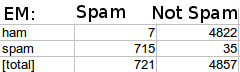
\includegraphics[width=0.93\columnwidth]{figures/EM.png}
\caption{ The result of the EM clustering and classification from left
  to right: the actual class of the instance, the number of instances
  classified as spam, and the number of instances classified as
  non-spam.  }
\end{figure}


\section{K Nearest Neighbor}


\begin{figure}[t]
\centering
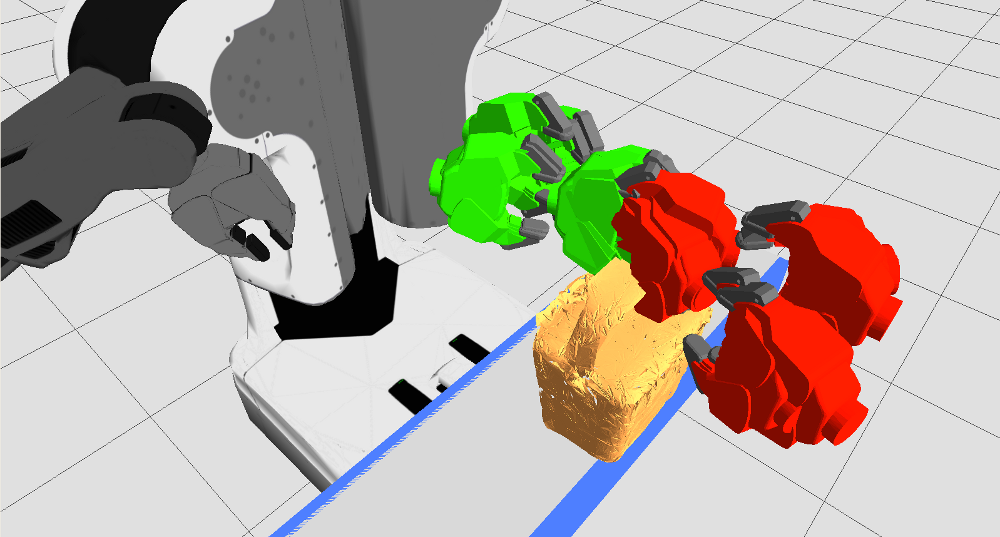
\includegraphics[width=\columnwidth]{figures/covered_basket-grasps-kinematics_check.png}
\caption{
The end-effectors in green are included in $X_{pg}$, while the ones shown in red are discarded by the kinematic feasibility check.
}
\label{fig:kinematics_feasibility_check}
\end{figure}

Given a set of valid grasps, a heuristic is typically used to select
the best grasp to plan for~\cite{WGGrasping}. However, this approach
can be overly restrictive, as the feasibility of the grasp depends on
the estimated time of arrival of the object. The better option is to
let the planner itself figure out which grasp to plan to given the
time constraint.
%a common approach to choosing which one to plan to, is to rank them using heuristics such as the number of sensed object points that fit inside the gripper or the distance from the object center~\cite{WGGrasping}. These heuristics are used because the grasp is planned on the fly and its quality is unknown. Given that our grasps were recorded previously, we are confident in their reliability and how to choose between them is unclear. 

% Thus, instead of choosing a single pregrasp-grasp tuple to target, the
% entire set of pregrasps in $X_{pg}$ is sent to the motion planner,
% allowing the planner to determine the $\{x_{p_j}, x_{g_j}\}$ in
% $X_{pg}$ that is feasible and optimizes costs well. After a plan is
% computed by the planner, the final waypoint of the planned path to the
% pregrasp, $x_{p_j}$, chosen by the planner. We use the corresponding
% grasp, $x_{g_j}$ as the grasp pose.

Thus, instead of choosing a single pregrasp-grasp tuple to target, the
entire set of pregrasps in $X_{pg}$ is sent to the motion
planner. When the planner finds a collision-free trajectory to an
element of $X_{pg}$, we select the corresponding grasp, $x_{g_j}$ as
the grasp pose. Computing the postgrasp is a straightforward process,
generic across object types. Given the grasp, $x_{g_j}$, we compute
the postgrasp, $x_{po_j}$, by searching through the set of postgrasps
for a kinematically feasible arm configuration that is as far from the
table as possible. In our experiments, we found that the $x_{po_j}$
chosen was typically within 12cm of $x_{g_j}$.

\subsection{Motion Planning}

% In an environment where robots work alongside people, it is important
% that the robot's behavior is consistent and predictable. This way, any
% human workers nearby can feel comfortable and safe around it. In
% particular, for a robot to be an effective member of a team on an
% assembly line that sorts moving objects into bins, the robot motions
% needs to be consistent, predictable and as close to optimal as
% possible in order for people to be able to work alongside and within
% the workspace of the robot. With this in mind, we implemented a
% heuristic search-based approach to generate motion plans for each of
% the robot's arms independently.

Heuristic searches such as A* provide strong theoretical guarantees
such as completeness and optimality or bounds on
suboptimality~\cite{Pearl-heur}. Their generality allows for complex
constraints and cost functions, while providing good cost minimization
and consistency in the solution. Consistency here implies that given
similar input, similar output is produced, thus making the robot's
motions more predictable.

Motion planning for pick-and-place of moving objects needs to be
performed as fast as possible so the robot has enough time to execute
the computed motions in time. To combat the high dimensionality of the
planning problem, we employ a heuristic search based approach that
uses an anytime variant of A* called ARA*~\cite{LikGorThr-ara} that
quickly finds an initial, and possibly sub-optimal, solution and
repairs it while deliberation time allows. The approach also relies on
a compact graph representation and informative heuristics to provide
real time performance. Details on this approach and applications to single and dual-arm motion planning can be found in~\cite{Cohen2, Cohen3}. 

We configured the planner to search in a 7 dimensional task space, $\{{x, y, z, roll, pitch, yaw, \theta}\}$, that represents the 6-DOF pose of the end-effector in the world frame, coupled with $\theta$, the position of the redundant degree of freedom in the robot's arm. This representation can be used when planning for a robot with one or more 7-DOF manipulators, such as the PR2 robot. In our experiments, we execute two independent instances of the planner, one for each arm. The cost function we use is aimed to minimize the 6-DOF path length of the end-effector.

During the pick action, the planner is called to plan a path from the \textit{waiting} configuration of the arm to one of the pregrasps in $X_{pg}$. Before planning begins, the geometry of the fixed objects in the robot's workspace are added to the collision representation. In our experiments, this included the conveyor belt and bins that surrounded the robot. After the robot grasps the object, the collision geometry of the object is attached to the robot's collision model. During the place action, a plan is requested from the postgrasp to any one of the drop poses above the bins. Note that there is nothing constraining the user from having the robot gently place the item on a surface instead. Now that a potentially fragile object (or an object filled with something) is grasped in the robot's end-effector, we impose an upright path constraint on the planner when computing a path for the place action. The constraint requires the planner to maintain the initial $\{roll, pitch, yaw\}$ of the end-effector throughout the path with a small tolerance in each dimension.
 
After a path is computed, we pass it through a simple deterministic shortcutting routine that can deal effectively with discretization artifacts. We found that only a single pass through the points was necessary. In our experiments, the entire shortcutting step lasted between 5-10ms, including checking the interpolated motions for collisions every $2^{\circ}$.

The ability to accurately predict the time it takes to execute a
trajectory is essential to picking up a quickly moving object. Being
that our motion planner plans solely for the kinematics of the arm, we
then perform a final post-processing step, in which the shortest
timing intervals between points are computed that enforce the robot's
dynamic constraints~\cite{IterativeSmoother}. The waypoint locations
themselves are not moved, instead feasible velocities and
accelerations are assigned. We found in our experiments that on
average, for a trajectory from an arm's initial configuration to a
pregrasp pose, the predicted execution timing and the actual
trajectory execution timing differ by approximately \unit[80]{ms}. The
pregrasp-to-grasp trajectory is much shorter, which provides for a
much smaller temporal prediction error, thus making the pregrasp pose
a useful waypoint at which to make final timing adjustments to achieve
a precise collision.

\subsection{Execution}

Given that the object is moving at a reasonable pace, the pick action
is substantially more difficult to execute than the place because very
precise timing is needed to succesfully pick up the object with a firm
grasp. For example, in our experiments the objects moved at
approximately \unitfrac[33]{cm\,}{\,s} across the robot's
workspace. At that velocity, if the execution of our grasp motion is
\unit[100]{ms} too late, the object will have passed $x_{pred}$ by
more than \unit[3]{cm}, and, depending on the type of the object, it
is very likely that the end-effector will swipe and miss.

\textit{\textbf{Pick Action.}} 
At this stage in the pipeline, it is confirmed that the entire pick action is kinematically feasible. In the case of the pick action, the following two trajectories have been generated:

\begin{itemize}
\item $traj_{p}$ - The pregrasp trajectory begins at the waiting configuration of the arm and ends at $x_{p_{j}}$. It is a collision free path generated by the motion planner, then shortcutted and filtered. $traj_{p}$ has a predicted trajectory execution duration of $d_{p_{pred}}$ seconds.
\item $traj_{g}$ - The grasp trajectory begins with the wrist at $x_{p_{j}}$, then moves to $x_{g_{j}}$ and ends at $x_{po_{j}}$. The path is an open loop motion in which the end-effector moves a very short total distance. $traj_{g}$ is filtered to assure the robot can execute it. Note that we define $d_{g_{pred}}$ as the predicted trajectory execution duration of the trajectory from the start until $x_{g_{j}}$. We disregard the execution time from $x_{g_{j}}$ to $x_{po_{j}}$ because the first half of the motion is the only time sensitive component, given that the end-effector has to be at $x_{g_i}$ to pick up the object at $x_{pred}$ at time $t_{pred}$.
\end{itemize}

The next step is to determine whether there is enough time for the
robot to execute both trajectories in time to pick up the object at
$t_{pred}$. The pickup is determined to be feasible if $t_{pred} >
(t_{now} + d_{p_{pred}} + d_{g_{pred}})$. If the pickup is feasible,
then $traj_{p}$ is executed immediatly. After it is completed,
$traj_{g}$ will begin execution at $t_{g_{execute}} = t_{pred} -
d_{g_{pred}}$. The end-effector is commanded to start closing as it is
approaching the grasp pose. In our experiments, we found that
depending on how early the object was detected and which arm is being
used, the robot would sleep for between 0.0 and 1.5 seconds between
executing the trajectories to ensure a well-timed grasp.


\textit{\textbf{Place Action.}}
After the object is grasped and raised to the postgrasp, there is not much work left to do. The computed path with the upright orientation constraint on the end-effector is executed immediatly. After the end-effector opens, allowing the object to drop into the desired bin, the arm returns to the waiting configuration. The purpose of the waiting configuration is two fold. First, it is intended to keep the arm that is closer to the feed edge of the belt out of the view of the RGB-D sensor, regardless of where the bins are located. Second, it is desirable to keep the arm in a configuration that is close to the table to aid in quicker reaction times by having to execute shorter trajectories.




\section{Experiments}

% We should have a \subsection{PR2 Robot} discussing the PR2. We should try to keep the paper as robot agnostic as possible and here we should have an introduction to our chosen mobile manipulation platform, the pr2.

\subsection{Computing Platforms}
All logic related to planning was executed onboard the PR2's own
computers. The perception software was hosted remotely on a desktop
computer with an Intel Core i7-2600 quad-core CPU at 3.4GHz and an
NVIDIA GeForce GT 420 GPU with 48 CUDA cores, a low-end graphics card
from 2010. The imposition of networking between these two critical
components adds a significant and variable amount of latency to the
system, however the PR2 used for these experiments did not have a
discrete GPU, and so could not host the perception system itself. The
perception pipeline was written in the Haskell functional programming
language, and compiled with the
GHC\footnote{\url{http://www.haskell.org/ghc}} 7.6.1 compiler.

\subsection{Object Selection}
\begin{figure}[t]
\centering
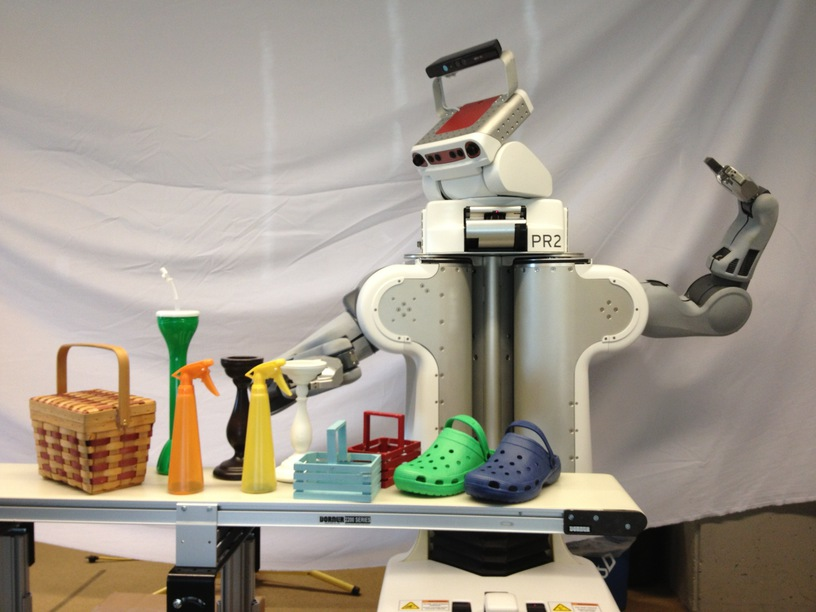
\includegraphics[width=0.8\columnwidth]{figures/object-group-photo-sm.jpg}
\caption{
The objects used for all experiments.
}
\label{fig:group-photo}
\end{figure}

The objects chosen, Figure~\ref{fig:group-photo}, range in height from
\unit[15]{cm} to \unit[45]{cm}, and breadth from \unit[8]{cm} to
\unit[25]{cm}. These objects also display a variety of rotational
symmetries, which affects their localization and how the objects may
be grasped. The candlesticks and tall green bottle have an infinite
order of rotational symmetry, denoted $C_\infty$, which translates to
a freedom to grasp such an object from any angle, and frees the
localization optimization from needing to consider object
orientation. The shoe is not rotationally symmetric, denoted $C_1$,
and must be grasped from its open end. The spritzer bottle is also
$C_1$, but may be grasped from either side to hook the PR2's fingers
underneath the overhanging geometry of the trigger mechanism. The
various baskets are all $C_2$, as their handles may be grasped from
either side.

Object models were acquired using RoboEarth software
\cite{DiMarco2012:RoboEarthModel}, a poster with fiducial markers, and
a Kinect sensor. The models gathered for the experiments described
here consist of 500 thousand to 1 million points.

\subsection{Pick-and-Place}
Figure~\ref{fig:group-photo} shows the conveyor belt used for testing
both static grasps, in which objects are placed on the surface in
front of the PR2 with the belt motor turned off, and dynamic grasps,
in which the belt motor is on. In the static grasp configuration, the
robot's head is oriented so that it is looking down at the table, and
objects are rapidly placed in front of it. As soon as the robot begins
to clear the work surface with an object in hand, a new object is
placed on the surface. Objects are placed such that at least one arm
can plausibly perform a grasp, but precise position and orientation
are allowed to vary within that constraint.

The experiment conducted in the static grasp configuration involved
100 pick-and-place operations in which the robot removes an object
placed onto the work surface in front of it, and places the object
into one of two bins placed on either side of it. Of the 100 attempted
actions, 91 were successful. The most common failure mode involved the
object slipping out of the robot's gripper due to an insecure
grasp. These 100 actions were timed in blocks of 10, yielding an
average of \unit[6.7]{s} per pick-and-place action. During the time
these experiments were conducted, the perception system failed to
identify an object before a two second timeout period elapsed on two
occasions. The experiments in which perception failed are not included
in the reported time, as we did not have a consistent approach to
failure recovery.

The dynamic configuration shown in the video associated with this
paper has the robot looking down the length of the conveyor belt, as
in Figure~\ref{fig:group-photo}. Objects are placed on the far end of
the \unit[2.13]{m} belt, and carried past the robot. In this
configuration, the perception system only reports on objects it has
seen a minimum of three times. This limits system responsiveness, but
is important to eliminate spurious observations of the object being
hand-placed on the end of the belt, and to ensure stability in pose
estimation.

System performance was measured over 100 pick-and-place operation
attempts with the belt at its top speed, \unitfrac[33]{cm\,}{\,s}, 87
of which were successful. Six objects were effectively ignored due to
the planner being unable to compute a suitable trajectory for either
arm in the allotted time. Of these six, five were spritzer bottles,
suggesting that the grasps chosen for this object did not leave the
planner enough freedom to maneuver. The seven other failures were
fumbled grasps. As in the static test, sometimes an insecure grasp
would lead to an object being dropped. The dynamic test added the new
failure mode of objects bouncing off of the back of the open gripper
during a catch attempt. This contribution of momentum to the
experiment was an excellent test of the system's overall timing: the
gripper had to close around the object as it hooked available geometry
in order to absorb all of its momentum without excessively
destabilizing the object. The tight timing constraints, paired with
the design of the PR2's arms, meant that the robot's arm farther from
where the objects were coming from was easier to utilize. Of the 94
attempted grasps, 57 were made by the far arm.

\section{Analysis}
\subsection{Perception Performance}
Preprocessing includes collecting a point cloud for each object to be
identified. The raw point data is used to populate a \unit[0.5]{cm$^3$}
resolution voxel grid, then passed through a Euclidean Distance
Transform (EDT), taking an average of \unit[304]{ms} for each object.

% \begin{figure}[t]
% \centering
% 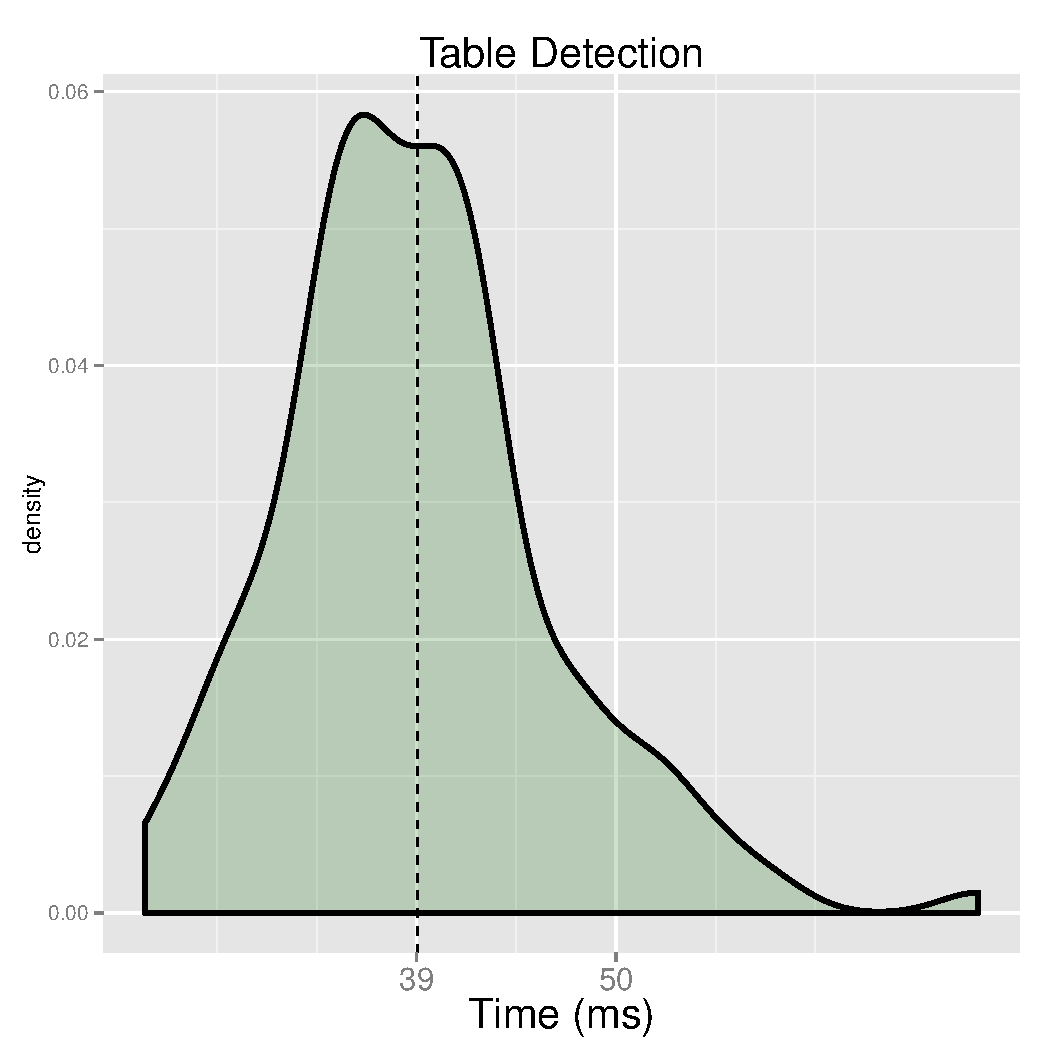
\includegraphics[width=0.8\columnwidth]{figures/table-density.pdf}
% \caption{
% Table extraction is performed with a recursive histogram over
% candidate connected components of the depth image.
% }
% \label{fig:table-density}
% \end{figure}

Once the system is running, parameters describing the conveyor belt
surface are periodically recalculated as described in
Section~\ref{sec:table-detection}. This process took an average of
\unit[39]{ms} per update, and was run concurrently with the rest of
the perception pipeline in a separate thread.

% Figure~\ref{fig:table-density}
% shows a kernel density estimate of overall table detection
% performance, with a mean processing time of 39ms. This process is run
% concurrently to the rest of the perception pipeline in a separate
% thread, and does not noticeably impact performance of the higher
% frequency components of the perception system.

\begin{figure}[t]
\centering
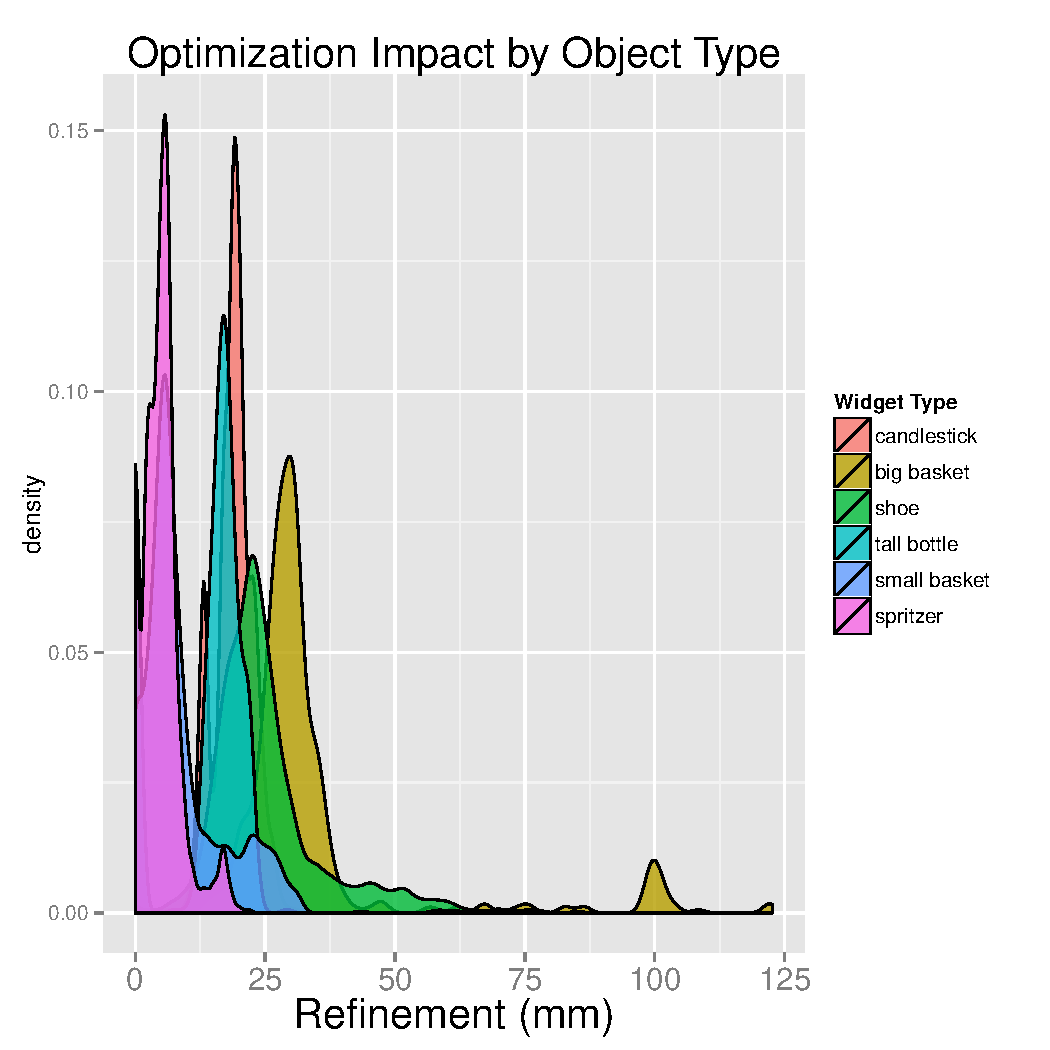
\includegraphics[width=\columnwidth]{figures/refinement.pdf}
\caption{
A nonlinear optimization that fits observed points to a per-object
cost function refines an initial localization estimate provided by
each point cluster's centroid.
}
\label{fig:refinement}
\end{figure}

The localization step begins by considering the centroid of each
cluster of points found above the table surface. This is a reasonably
good estimate of the object's position, but is biased towards the
camera due to self-occlusion of the object geometry. The goal of
navigating the PR2's finger into an opening with approximately
\unit[1]{cm} clearance on either side (e.g. underneath a spritzer
bottle's trigger) demands a level of accuracy in object pose
estimation which can be difficult to achieve when using only point
cluster centroids. However, the localization refinement step
represents a significant fraction of all the time spent in perception,
so its utility is of interest. Recovering object yaw is critical for
grasping asymmetric objects, but focusing solely on translational pose
estimation reveals further contributions made by refining initial
coarse position estimates.

Figure~\ref{fig:refinement} illustrates the translation corrections
made by the optimizer to an initial localization estimate based on
point cluster centroids with a kernel density estimate of observed
refinements. Note that in this run of experiments, there were no false
identifications and no wild misses by the robot. The two object types
needing the greatest correction from their initial centroid estimates
were the big basket and the shoe, which are the two objects with the
greatest asymmetry in the XY plane. The big basket is also a tall
object, resulting in views looking down the table that primarily see
the near side of the object. In contrast, most of the perimeter of an
item like the small basket could be seen at the available view
angle. This contrast is borne out by the effect of the optimization on
these two objects: the big basket's translational position was shifted
an average of \unit[3.4]{cm} from the point cluster centroid, while the small
basket was shifted an average of \unit[0.9]{cm}.

% \begin{table}[t]
% \centering
% \begin{tabular}{|c|c|}
% \hline
% Perception Stage & Mean Time (ms)\\ \hline \hline
% Table Extraction & 39.0 \\ \hline\hline
% Cloud Clustering & 22.2 \\ \hline
% Localization & 31.1 \\ \hline
% Total Perception & 53.2 \\ \hline
% \end{tabular}
% \caption{Perception Timing}
% \label{tab:perception-timing}
% \end{table}

\begin{figure}[t]
\centering
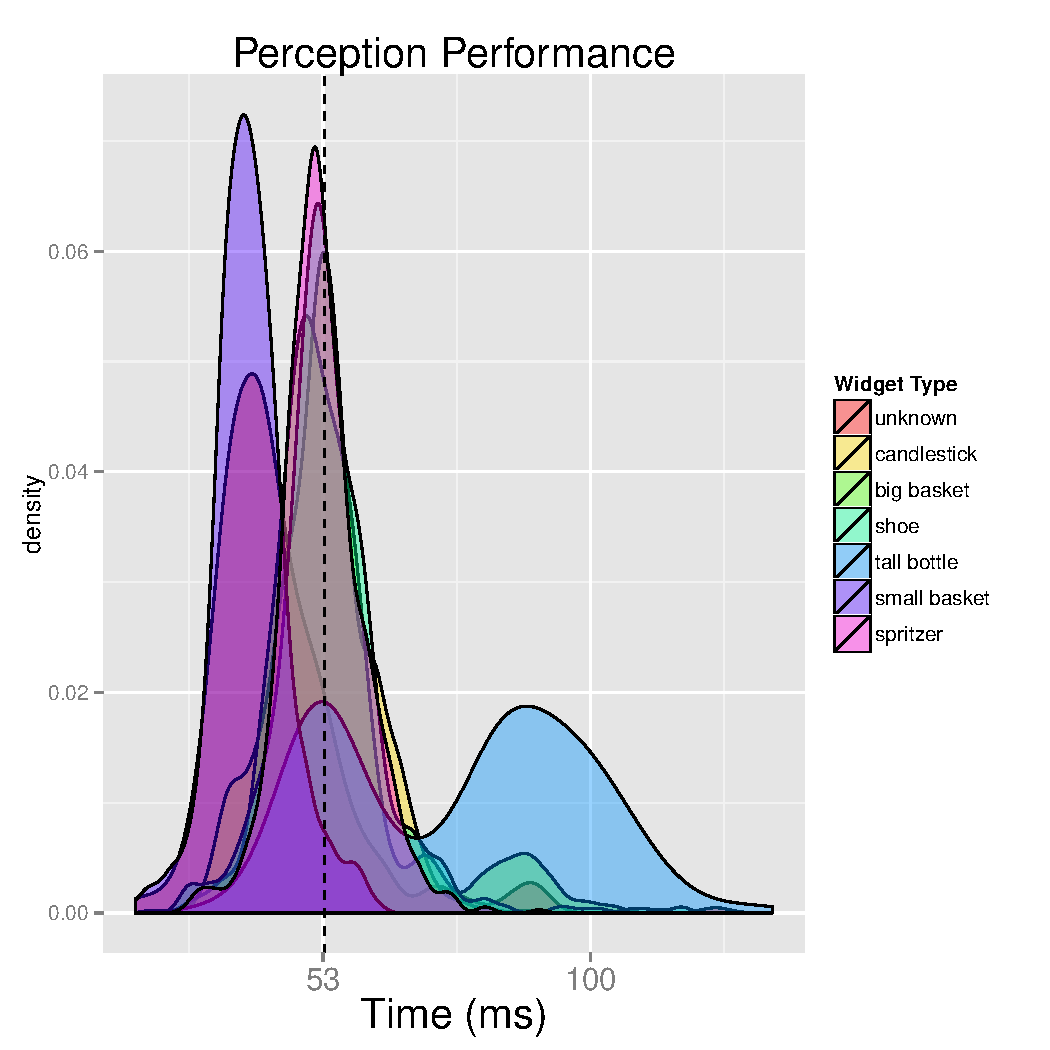
\includegraphics[width=\columnwidth]{figures/perception-density.pdf}
\caption{ Perception performance broken down by object type. The
  overall mean is \unit[53]{ms}.  }
\label{fig:perception-density}
\end{figure}

The average processing time for the perception system over the 5117
object detections during the moving object experiment was
\unit[53]{ms}, Figure~\ref{fig:perception-density}. The ``\textit{tall
  bottle}'' object was the slowest to process, at an average of
\unit[77]{ms} per update. Initial filtering, clustering, and coarse
recognition comprise the first perception phase, taking an average of
\unit[22.2]{ms}. The second phase consists of the localization
optimization procedure, taking an average of \unit[31.1]{ms}. The
final tracking phase did not take a significant amount of time.

The average processing time for the motion planner during the moving
object experiment was \unit[182]{ms}, including time spent in ROS
service calls. This gives a minimum system response time on the order
of \unit[250]{ms} if only one observation of a scene is needed. For
applications such as dynamic object manipulation, multiple
observations may be needed, which pushes the delay before action to
over \unit[400]{ms}. The performance of these experiments is thus
completely dominated by the speed at which the PR2 can move its
arms. The PR2 requires approximately \unit[4.5]{s} to perform the
motions needed for these tasks, which puts a lower limit on how
quickly the entire system can process pick-and-place tasks.

\subsection{Robustness}
Execution time -- a limiting factor in system responsiveness -- was
consistent throughout the experiments described. The longest single
perception update in the dynamic test covering 5117 updates took
\unit[132]{ms}. There are many sources of variance in these timings as
the perception system was running on the GHC Haskell runtime system
with its generational garbage collector, which itself was running in a
desktop Linux environment (Ubuntu 10.04).

Localization accuracy was measured by considering the PR2's effective
``hand-eye coordination.'' We used the PR2's proprioception to obtain
an estimate of the location of one of the robot's fingertips with its
arm extended over the work surface and angled down so that the finger
just touched the surface. The location of this tangent was marked, and
the arm was removed from the work area. A candidate object was then
placed at the marked location, and the localization returned by the
perception system was compared with the PR2's own estimate of where
its finger had been. 

These experiments yielded an average discrepancy between
proprioception and perception of \unit[5.3]{mm}. A meter stick was
then used to move the object one meter down the work surface from its
starting location. The robot's head was turned to face this new
location, and the output of perception was again recorded. This
relative motion estimate yielded an average discrepancy between the
meter stick and the perception system of \unit[6.7]{mm}.

The last metric recorded from the perception system was the speed of
the belt. This was estimated during the experiment by tracking objects
over time. The perception system estimated the belt speed at
\unitfrac[33.1]{cm\,}{\,s}, with a standard deviation of
\unitfrac[0.08]{cm\,}{\,s}. We were unable to obtain another
measurement of belt speed with less noise.

The reported timings include all segmentation, recognition, and
localization. There is additional overhead in the integrated system
due to running the perception calculations remotely from the PR2
itself. The net result was a ROS object detection publisher rate that
varied between 10 and \unit[12]{Hz}, the same rate at which raw depth
images were received at the perception computer.

\section{Conclusion}
We have demonstrated pick-and-place operations performed by a PR2 at a
rate of \unit[6.7]{s} per object at a 91\% success rate. Similar
operations on a moving work surface yield an 87\% success rate. Room
for improvement remains in the areas of system integration, and
end-effector customization. The speed at which the PR2's arms can move
proved to be a limiting factor in system performance, and the gripper
design was not particularly suited to absorbing the impact of moving
objects. Despite these mechanical limitations, the PR2 proved to be
capable of responsive, high throughput object manipulation.

\section{Acknowledgements}
This research was in part sponsored by the Army Research
Laboratory Cooperative Agreement Number W911NF-10-2-0016.


\bibliographystyle{IEEEtran}
\bibliography{refs}
\end{document}
